\section{Language Model Design}
\label{sec:implementation}

\subsection{Model Architecture}
To better adapt to our proof-guided synthesis system and maximize token utilization efficiency, we design a novel encoder-decoder-based model architecture, illustrated in \autoref{fig:model-arch}.

Unlike standard encoder-decoder models that encode only a static input, our architecture features a \emph{dual-encoding} design that separately processes two distinct input streams: (1) the fixed natural language specification, and (2) the dynamically evolving synthesis goal at each step.

\paragraph{Static Encoding.} The natural language specification remains unchanged throughout the synthesis process. We encode it once at the beginning to produce a fixed sequence of hidden states that stays constant across all synthesis steps.

\paragraph{Dynamic Encoding.} The synthesis goal, which provides the \emph{dynamic typing context}, evolves at each step as the synthesis derivation tree grows. We re-encode the current synthesis goal at each step to capture the updated typing context. The encoder produces a separate sequence of hidden states for this dynamic input.

\paragraph{Cross-Attention Fusion.} The decoder accesses both encodings through cross-attention mechanisms. We concatenate the static encoding $H_s$ and dynamic encoding $H_d$ along the sequence dimension to form a unified key-value sequence $H = [H_s; H_d]$. The decoder's cross-attention layers then attend to this concatenated sequence, computing attention over both the task specification and the current typing context simultaneously. This design allows the model to jointly reason about both information sources when predicting the next synthesis decision.

\begin{figure}[t]
\centering
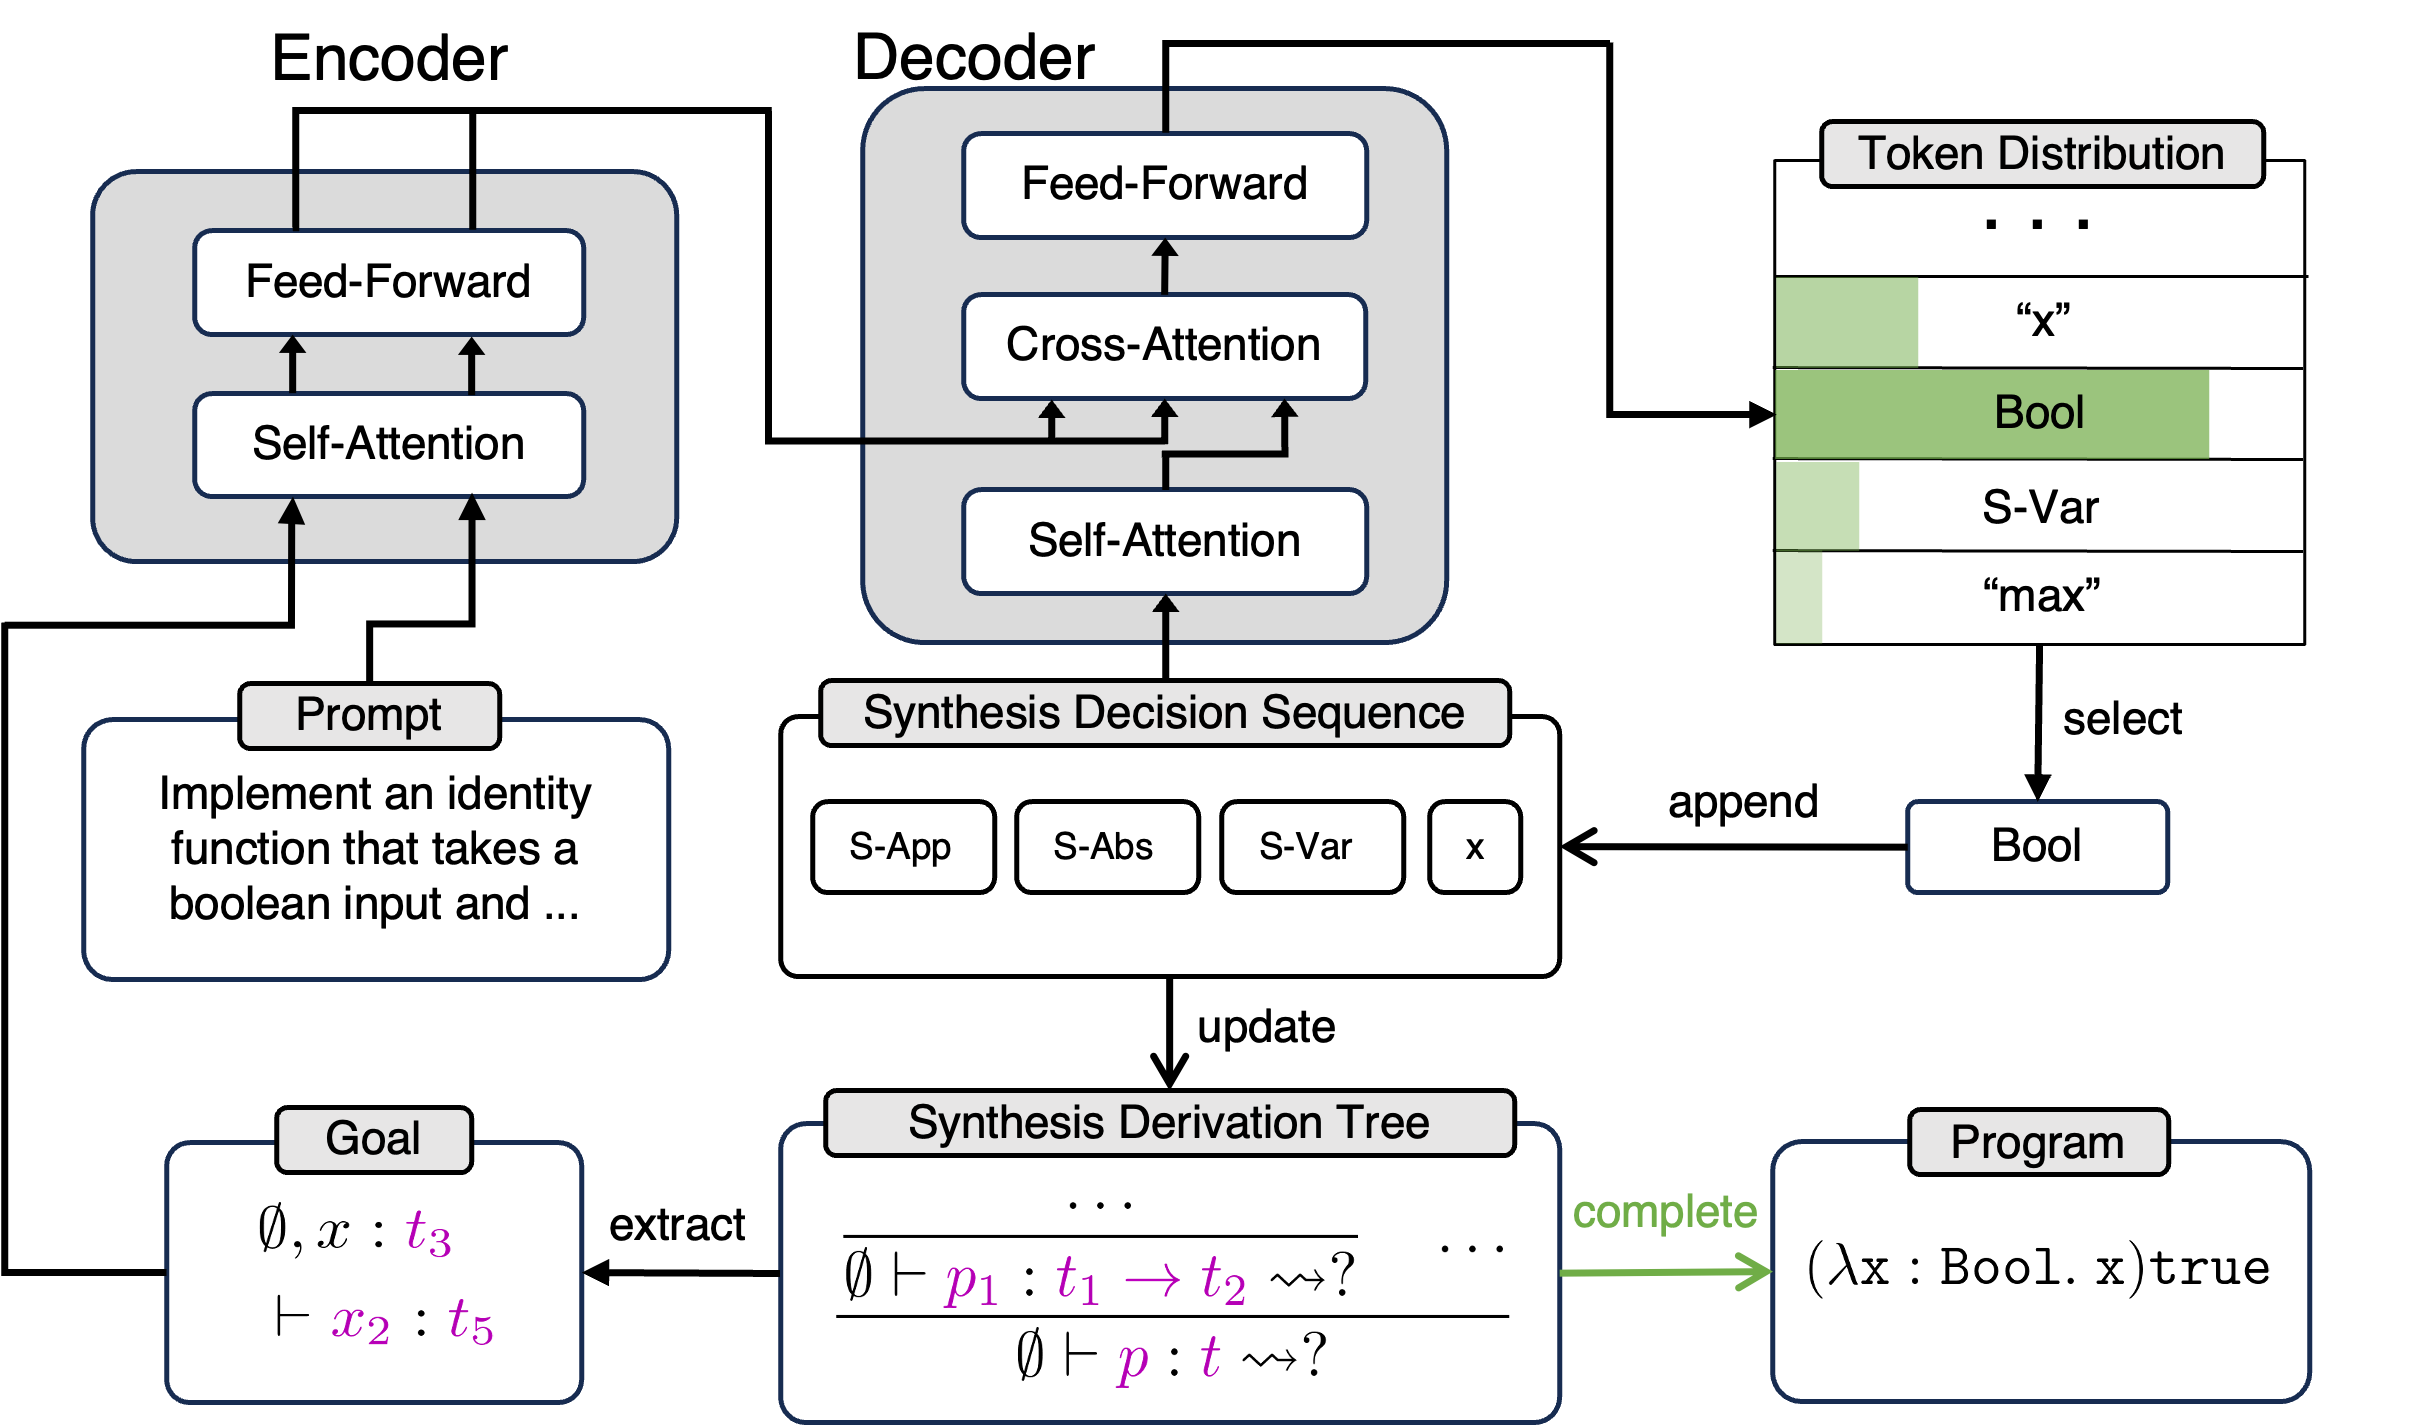
\includegraphics[width=0.9\textwidth]{assets/model_arc2.png}
\caption{Model Architecture for Constructing Synthesis Derivation Trees}
\label{fig:model-arch}
\end{figure}

As described in \autoref{sec:query-resolution-lm}, the query resolution task is delegated to the LM, which takes the natural language prompt, the synthesis decisions generated so far, and the current synthesis goal as input and outputs a token representing the synthesis rule or variable assignments.

Meanwhile, \mainname maintains a synthesis decision sequence where each newly generated token is appended, representing the next synthesis decision. This sequence incrementally constructs an existential type correctness proof. Due to its autoregressive nature, the growing sequence is fed to the transformer decoder, allowing the LM to leverage the full history of synthesis decisions when predicting the next token.

\paragraph{Model Inference Process.}
At each synthesis step:
\begin{enumerate}
    \item The current synthesis goal is extracted from the (incomplete) synthesis derivation tree.
    \item The encoder encodes the synthesis goal to provide \emph{dynamic typing context} to the LM.
    \item The decoder processes both encodings from the encoder, along with the previous synthesis decision sequence, generating the next token representing a synthesis decision.
    \item This new token is appended to the synthesis decision sequence and used to incrementally update the synthesis derivation tree as detailed in  \autoref{alg:synthtree}.
    \item The updated synthesis derivation tree yields either a new synthesis goal for the next iteration or, upon completion, a well-typed program together with its type correctness proof.
\end{enumerate}

\paragraph{Efficient Token Reuse through Incremental Construction.}
According to \autoref{alg:synthtree}, the synthesis derivation tree construction follows a serialized order, ensuring that each step only appends new decisions without modifying the existing sequence.
This property aligns naturally with the autoregressive generation paradigm of transformer decoders, where each new token is predicted based on all previously generated tokens.
%
As a result, we can reuse the transformer's key-value (KV) cache~\cite{DBLP:conf/mlsys/PopeDCDBHXAD23}: the intermediate attention states computed for earlier tokens in the decision sequence are cached and reused when generating subsequent tokens. This eliminates the need to recompute attention over the entire decision sequence at each decision-making step, significantly reducing the computational overhead from quadratic to linear in sequence length.

\paragraph{Model Configuration.}
Our dual-encoding architecture is built upon standard Transformer encoder-decoder models, where both the encoder and decoder follow the standard Transformer architecture~\cite{DBLP:conf/nips/VaswaniSPUJGKP17}. We evaluate on two pre-trained models: \textbf{CodeT5-220M}~\cite{DBLP:conf/emnlp/0034WJH21}, with 12-layer encoder and 12-layer decoder, 12 attention heads, a hidden dimension of 768, and approximately 220 million parameters; and \textbf{T5Gemma2-2B}~\cite{zhang2025t5gemma2seeingreading}, with 26-layer encoder and 26-layer decoder, 8 attention heads, a hidden dimension of 2304, and approximately 2 billion parameters. For both models, the static encoder and dynamic encoder share the same weights but process different input streams.

\subsection{Term Encoding}
\label{sec:term-encoding}
Terms, as defined in \autoref{terms-intro}, are inductively constructed from constants and constructors. Following the approach of GrammarT5~\cite{DBLP:conf/icse/ZhuL000C24}, we serialize the abstract syntax tree (AST) of a term using a pre-order traversal, outputting each constructor or constant as a token in sequence. When a term contains unknown variables (not yet instantiated during synthesis), we represent them using a unified unknown token $\langle?\rangle$.

For example, consider the STLC program $\tcode{abs}(\tcode{"x"}, \tcode{bool}, \tcode{var}(\tcode{"x"}))$, which represents the identity function $\lambda x{:}\tcode{bool}.\, x$. Its AST has the constructor $\tcode{abs}$ at the root, with three children: the constant $\tcode{"x"}$ (the variable name), the constant $\tcode{bool}$ (the type annotation), and the subtree $\tcode{var}(\tcode{"x"})$. The pre-order traversal yields the token sequence illustrated in \autoref{fig:term-encoding}.

\begin{figure}[tb]
\centering
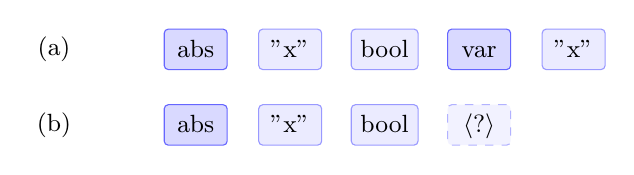
\begin{tikzpicture}[x=1.2cm, y=0.8cm]
    \tikzset{
        ctor/.style={
            draw=blue!60, fill=blue!15,
            minimum height=5mm, minimum width=8mm,
            rounded corners=1.5pt, font=\small,
            text depth=0.25ex, text height=1.6ex
        },
        const/.style={
            draw=blue!40, fill=blue!8,
            minimum height=5mm, minimum width=8mm,
            rounded corners=1.5pt, font=\small,
            text depth=0.25ex, text height=1.6ex
        },
        unknown/.style={
            draw=blue!30, fill=blue!5,
            minimum height=5mm, minimum width=8mm,
            rounded corners=1.5pt, font=\small,
            text depth=0.25ex, text height=1.6ex,
            dashed
        },
    }

    % ==== Full term encoding ====
    \node at (-1.5, 0) {\small (a)};
    \node[ctor] (c1) at (0,0) {\tcode{abs}};
    \node[const] (c2) at (1,0) {\tcode{"x"}};
    \node[const] (c3) at (2,0) {\tcode{bool}};
    \node[ctor] (c4) at (3,0) {\tcode{var}};
    \node[const] (c5) at (4,0) {\tcode{"x"}};

    % ==== Partial term encoding with unknown ====
    \node at (-1.5, -1.2) {\small (b)};
    \node[ctor] (p1) at (0,-1.2) {\tcode{abs}};
    \node[const] (p2) at (1,-1.2) {\tcode{"x"}};
    \node[const] (p3) at (2,-1.2) {\tcode{bool}};
    \node[unknown] (p4) at (3,-1.2) {$\langle?\rangle$};

\end{tikzpicture}

\setlength{\fboxsep}{1pt}
\caption{Term encoding as token sequences: 
\colorbox{blue!15}{\textsf{constructors}} and 
\colorbox{blue!8}{\textsf{constants}}.
(a) Full term $\tcode{abs}(\tcode{"x"}, \tcode{bool}, \tcode{var}(\tcode{"x"}))$.
(b) Partial term $\tcode{abs}(\tcode{"x"}, \tcode{bool}, \sk{e})$ with unknown variable.}
\label{fig:term-encoding}
\end{figure}

This encoding preserves the structural information of the term and can be uniquely decoded back to the original AST. The decoding is possible because each constructor has a fixed arity and known parameter types (as specified in the term definitions in \autoref{terms-intro}). When the decoder encounters a constructor token, it knows exactly how many subsequent tokens to consume and what types they should have, enabling unambiguous reconstruction of the tree structure. If the number of arguments or their types do not match the constructor's specification, the decoding fails and reports an error. During synthesis, the LM generates tokens following this same pre-order traversal order to construct terms for variable assignments. As each token is generated, the synthesis system incrementally decodes the sequence to reconstruct the corresponding AST, enabling immediate validation and integration into the synthesis derivation tree.

\subsection{Advanced Techniques for LM-Based Program Synthesis}
The program synthesis algorithm in \autoref{alg:synthtree} involves sequential actions at each node: selecting synthesis rules, acquiring variable assignments, and applying rules to update the synthesis derivation tree. 
%
To ensure the efficiency and correctness of this process, we implement pruning strategies that naturally correspond to the potential failures in synthesis rule application. 

At the syntactic level, we apply \emph{syntactic pruning}, which ensures the structural validity of synthesis derivation trees and enforces the well-formedness of generated sequences.
\emph{Syntactic pruning} is triggered instantly when a token is generated: (1) the synthesis goal expects a synthesis rule to apply but the token stands for a term, or vice versa; (2) the predicate in the synthesis rule's conclusion differs from that of the synthesis goal; or (3) during term generation, the token corresponds to constructors or constants (see \autoref{terms-intro}) that mismatch the expected term type.
%
\begin{example}
Consider generating the term $\tcode{abs}(\tcode{"x"}, \tcode{bool}, \tcode{var}(\tcode{"x"}))$ using the term encoding from \autoref{sec:term-encoding}. Suppose the current token sequence is $[\tcode{abs}, \tcode{"x"}]$, meaning the LM has generated the constructor $\tcode{abs}$ and its first argument $\tcode{"x"}$ (the variable name). According to the constructor specification $\tcode{abs} : (\tcode{String}, \tcode{Type}, \tcode{Prog})$, the next token should be of type $\tcode{Type}$. If the LM generates $\tcode{var}$ (a $\tcode{Prog}$ constructor) instead of a valid type like $\tcode{bool}$, syntactic pruning immediately rejects this token because the expected type $\tcode{Type}$ does not match the actual type $\tcode{Prog}$.
\end{example}

At the type level, we apply \emph{type pruning}, which focuses on type-level correctness and relies on premise checking during the application of synthesis rules. 
If the unification step or constraint checking step fails, the corresponding search is immediately terminated. 
This prevents the exploration of synthesis paths that cannot lead to valid type correctness proofs.
%
\begin{example}
Consider applying the \rulename{T-Var} rule, which has a constraint $\checkBinding{\Gamma}{x}{t}$ that checks whether the variable $x$ with type $t$ exists in the context $\Gamma$. Suppose the current synthesis goal is $\stlctype{\Gamma}{\sk{e}}{\tcode{int}}$ where $\Gamma = \{f : \tcode{bool}, g : \tcode{int}\}$. If the LM selects $f$ to instantiate $\sk{e}$, the constraint checking step verifies $\checkBinding{\Gamma}{f}{\tcode{int}}$. Since $f$ has type $\tcode{bool}$ in $\Gamma$, not $\tcode{int}$, the constraint fails and type pruning terminates this branch. The correct choice would be $g$, which has the matching type $\tcode{int}$.
\end{example}

\emph{Syntactic pruning}, \emph{type pruning}, and the previously mentioned \emph{dynamic typing context} constitute a layered enhancement framework: 
\emph{syntactic pruning} serves as a prerequisite for \emph{type pruning}, since a structurally invalid synthesis derivation cannot be applied to perform type-level checking. 
Furthermore, without the successful application of synthesis rules, the intended synthesis goal cannot be extracted from the synthesis derivation tree. 
Should all three techniques be omitted, the model reduces to a standard encoder-decoder architecture that directly maps natural language inputs to sequences of synthesis decisions, lacking any mechanism to enforce structural or type-level correctness.

Beam search~\cite{DBLP:conf/aclnmt/FreitagA17} enables efficient exploration of multiple synthesis paths by maintaining the top-$k$ candidate sequences based on cumulative likelihood scores. At each step, rather than greedily selecting only the highest-probability token, beam search expands all $k$ beams and retains the top-$k$ sequences across all candidates.
When a branch is pruned due to syntactic or type errors, we terminate its sequence and discard its KV cache, while remaining branches continue independently. This prevents invalid branches from wasting beam slots, ensuring all $k$ slots are reserved for branches that may lead to valid programs.